\documentclass[notitlepage, 12pt, reqno]{amsart}
\usepackage{amssymb}
\usepackage{amsmath}
\usepackage{tikz}
\usetikzlibrary{arrows.meta}
\usetikzlibrary{decorations.pathmorphing}
\usepackage{pgfplots}
\pgfplotsset{compat=newest}
\usepackage{color}

\begin{document}

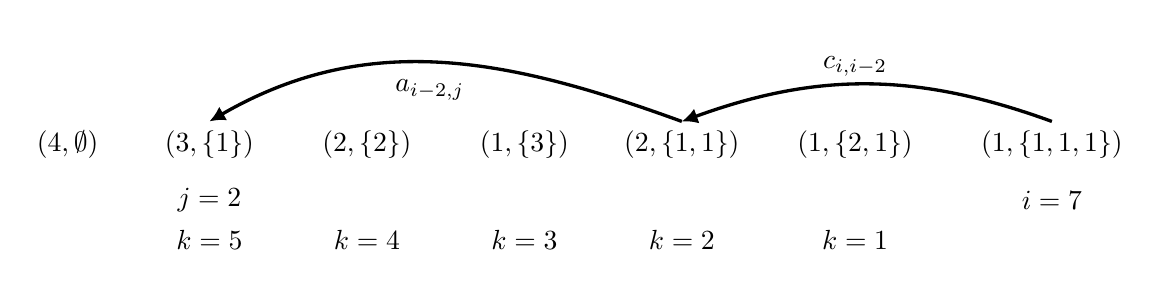
\begin{tikzpicture}
\node[] at (-58mm,0mm) {$(4, \emptyset)$};

\node[] at (-40mm,0mm) {$(3, \{1\})$};
\node[] at (-40mm,-7mm) {$j = 2$};
\node[] at (-40mm,-12mm) {$k = 5$};

\node[] at (-20mm,0mm) {$(2, \{2\})$};
\node[] at (-20mm,-12mm) {$k = 4$};

\node[] at (0mm,0mm) {$(1, \{3\})$};
\node[] at (0mm,-12mm) {$k = 3$};

\node[] at (20mm,0mm) {$(2, \{1,1\})$};
\node[] at (20mm,-12mm) {$k = 2$};

\node[] at (42mm,0mm) {$(1, \{2,1\})$};
\node[] at (42mm,-12mm) {$k = 1$};

\node[] at (67mm,0mm) {$(1, \{1,1,1\})$};
\node[] at (67mm,-7mm) {$i = 7$};

\draw[-{Latex[length=2mm, width=2mm]}, black, very thick] (67mm,3mm) to[out=160,in=20] (20mm,3mm);
\node[] at (42mm,10mm) {$c_{i, i - 2}$};

\draw[-{Latex[length=2mm, width=2mm]}, black, very thick] (20mm,3mm) to[out=160,in=30] (-40mm,3mm);
\node[] at (-12mm,7mm) {$a_{i - 2, j}$};

\end{tikzpicture}

\end{document}